\documentclass[12pt, a4paper]{article}
\usepackage[a4paper, top=2cm, bottom=2cm, left=3cm, right=1cm]{geometry}
\usepackage[T2A]{fontenc}
\usepackage[utf8]{inputenc}
\usepackage[russian]{babel}
\usepackage{listingsutf8}
\usepackage{float}
\usepackage{graphicx}
\usepackage{mathtools}
\usepackage{amsmath}
\usepackage{xcolor}

\graphicspath{{images/}}

% \mathtoolsset{showonlyrefs}

\definecolor{codegreen}{rgb}{0,0.6,0}
\definecolor{codegray}{rgb}{0.5,0.5,0.5}
\definecolor{codepurple}{rgb}{0.58,0,0.82}
\definecolor{backcolour}{rgb}{0.95,0.95,0.92}


\lstdefinestyle{mystyle}{
	backgroundcolor=\color{backcolour},   
	commentstyle=\color{codegreen},
	keywordstyle=\color{magenta},
	numberstyle=\tiny\color{codegray},
	stringstyle=\color{codepurple},
	basicstyle=\ttfamily\footnotesize,
	breakatwhitespace=false,         
	breaklines=true,                 
	captionpos=b,                    
	keepspaces=true,                 
	numbers=left,                    
	numbersep=5pt,                  
	showspaces=false,                
	showstringspaces=false,
	showtabs=false,                  
	tabsize=4
}

\lstset{inputencoding=utf8/koi8-r, style=mystyle}
\begin{document}
	
	\begin{titlepage}
		\centering{
			\MakeUppercase{\textbf{БЕЛОРУССКИЙ ГОСУДАРСТВЕННЫЙ УНИВЕРСИТЕТ}} \\[0.4cm]
			
			Факультет прикладной математики и информатики \\[0.4cm]
			
			\vspace{15em}
			
			{\large\bfseries{Отчёт по лабораторной работе №3}}
			
			{\large\bfseries{<<Интерполяционный кубический сплайн>>}} \\[4cm]
			
			\noindent
			\begin{tabular}{p{0.6\textwidth}p{0.6\textwidth}}
				& Выполнил: \\
				& Пищулёнок М.\,С. \\[1cm]
				& Преподаватель: \\
				& Горбачева Ю. Н.
				
			\end{tabular}
			
			\vfill
			
			{\normalsize Минск, 2020}
			
		}
	\end{titlepage}
	
\tableofcontents
	
\section{Постановка задачи}

Вычислить значения заданной функции $f(x)$ в узлах интерполяции 
$x_i = a+ih, i = \overline{0,n}$ на отрезке $[a,b]$ с шагом $h = \frac{b-a}{n}$.
По полученной таблице ${x_,, f(x_i)}$ построить интерполяционный кубический сплайн 
$S_3(x)$ с дополнительными условиями:

	\begin{equation}
		S_3'(a) = f'(a),\ S_3'(b) = f'(b)
		\label{eq:condition_1}
	\end{equation}

	\begin{equation}
		S_3''(a) = f''(a),\ S_3''(b) = f''(b)
		\label{eq:condition_2}
	\end{equation}

	\begin{equation}
		S_3''(a)=0,\ S_3''(b) = 0
		\label{eq:condition_3}
	\end{equation}

Убедиться, что значения функций у узлах интерполяции совпадают со значениями 
сплайна для всех типов дополнительных условий. В точках
 $\overline{x_j} = a+(j+0.5)h$, $j=\overline{0, n-1}$ вычислить значения сплайна
 для всех типов дополнительных условий и сравнить со значениями функции $f(x)$ в
 этих точках, т.е. найти 
 
 \begin{equation}
	\max_{j=0,\ n-1}|f(\overline{x_j}) - S_3(\overline{x_j})|
	\label{eq:criteria}
 \end{equation}

 В одной системе координат построить график функции $f(x)$  и графики кубического 
 сплайна для трёх типов дополнительных условий.

 \begin{equation}
	 f(x) = \frac{x^2}{1+x^3},\ n=15,\ a=0,\ b=2
 \end{equation}
	
\section{Теория}

Кубический сплайн имеет вид:

\begin{equation}
	P_{i,3}(x) = a_i + b_i(x-x_{i-1}) + c_i(x-x_{i-1})^2 + d_i(x-x_{i-1})^3
\end{equation}

Коэффициенты $a_i,\ b_i,\ c_i,\ d_i$ находится из соотношений

\begin{align}
	a_i &= f(x_{i-1}) \\
	b_i &= \frac{f(x_i) - f(x_{i-1})}{h} - \frac{2c_i + c_{i+1}}{3}h \\
	c_{i-1} + 4c_i + c_{i+1} &= 3\frac{f(x_{i-2}) - 2f(x_{i-1} + f(x_i))}{h^2},\ i=\overline{2, n} \\
	d_i &= \frac{c_{i+1} - C_i}{3h}
\end{align}

\begin{enumerate}
	\item $S_3'(a) = f'(a),\ S_3'(b) = f'(b)$
	
	\begin{align}
		2c_1 + c_2 &= 3\frac{f(x_1) - f(x_0)}{h^2} - 3\frac{f'(x)}{h} \\
		c_n + 2c_{n+1} &= 3\frac{f'(b)}{h} - 3\frac{f(x_n) - f(x_{n-1})}{h^2}
	\end{align}

	\item $S_3''(a) = f''(a),\ S_3''(b)=f''(b)$
	
	\begin{equation}
		c_1 = \frac{f''(a)}{2},\ c_{n+1} = \frac{f''(b)}{2}
	\end{equation}
	
	\item $S_3''(a) = 0,\ S_3''(b) = 0$
	
	\begin{equation}
		c_1 = c_{n+1} = 0
	\end{equation}

\end{enumerate}

\section{Программа}

\lstinputlisting[language=python]{solution.py}
	
\section{Результаты}

\begin{figure}[H]
	\centering
	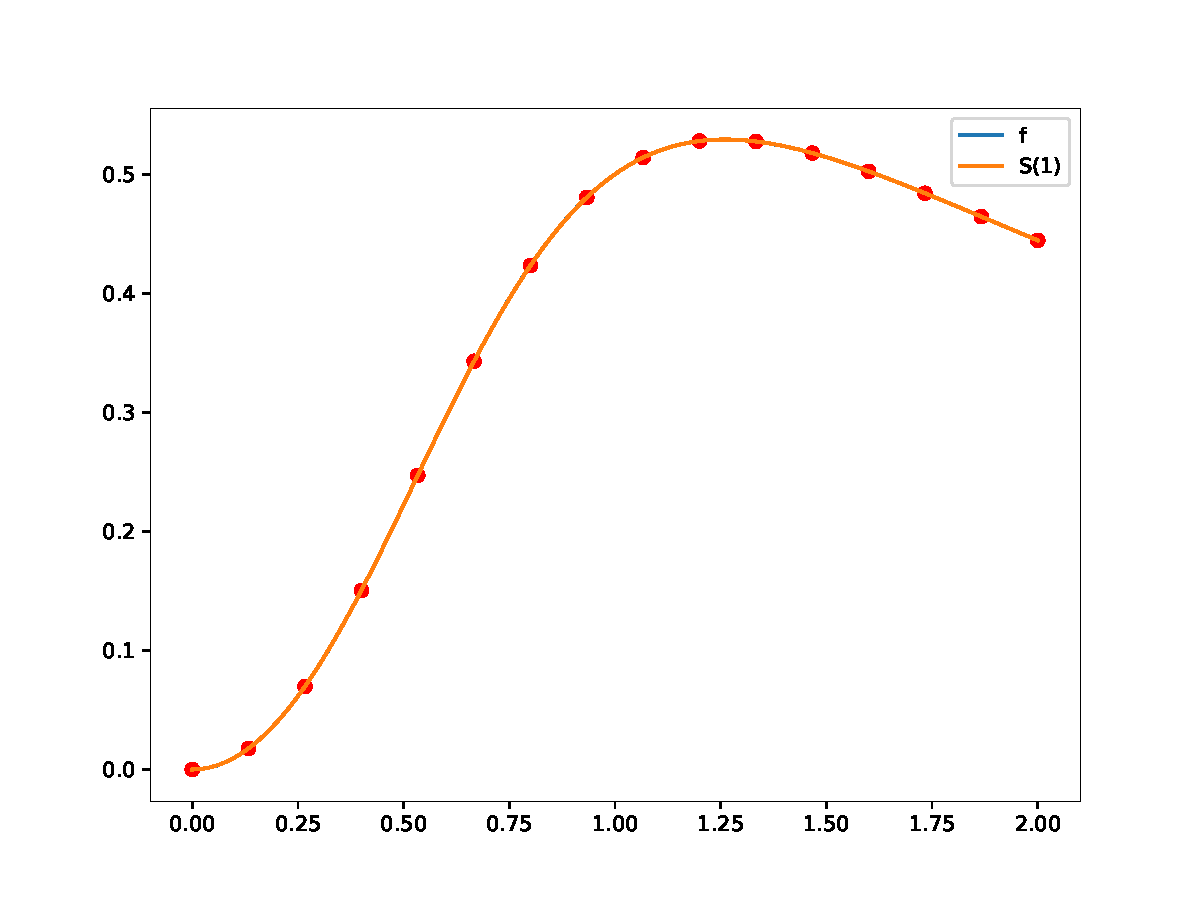
\includegraphics[width=\linewidth]{1.pdf}
	\caption{Первое дополнительное условие}
	\label{fig:case_1}
\end{figure}


\begin{figure}[H]
	\centering
	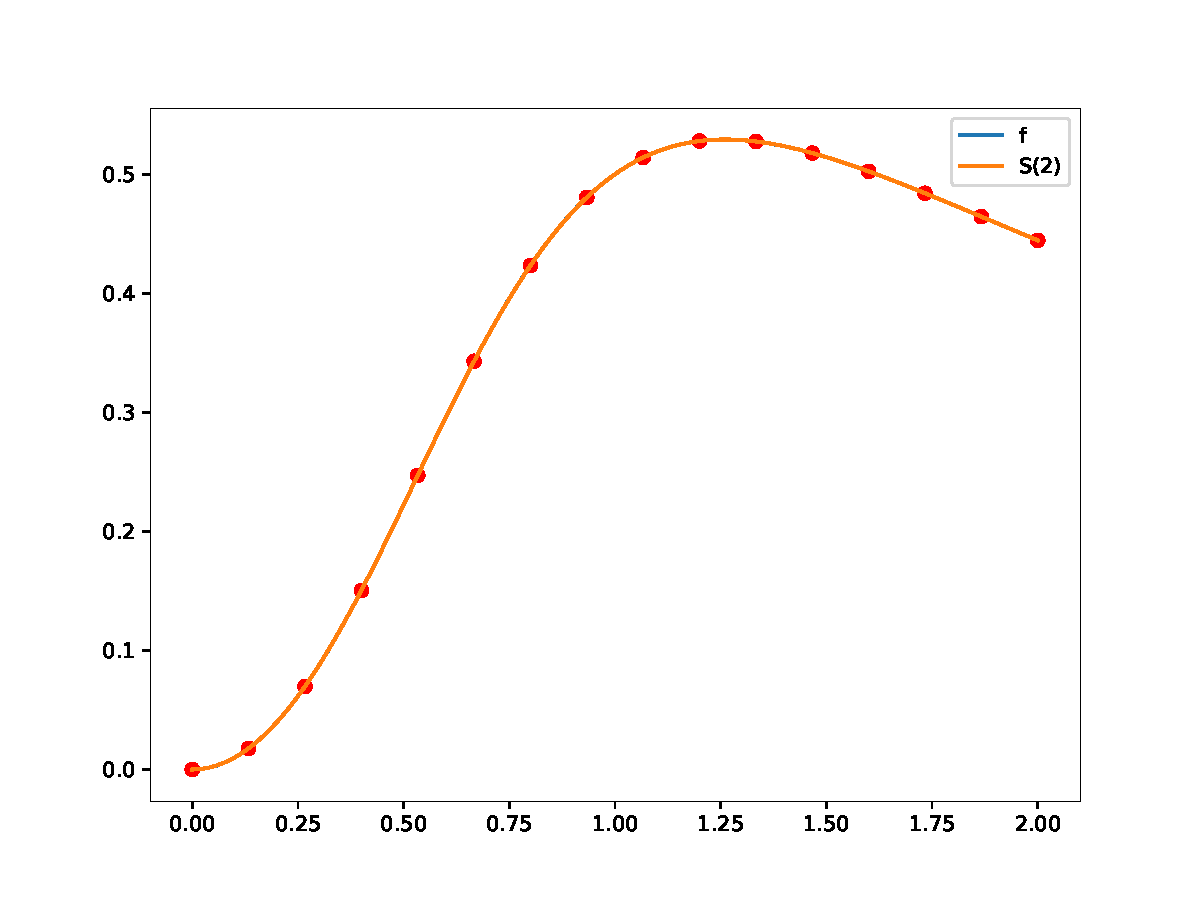
\includegraphics[width=\linewidth]{2.pdf}
	\caption{Второе дополнительное условие}
	\label{fig:case_2}
\end{figure}



\begin{figure}[H]
	\centering
	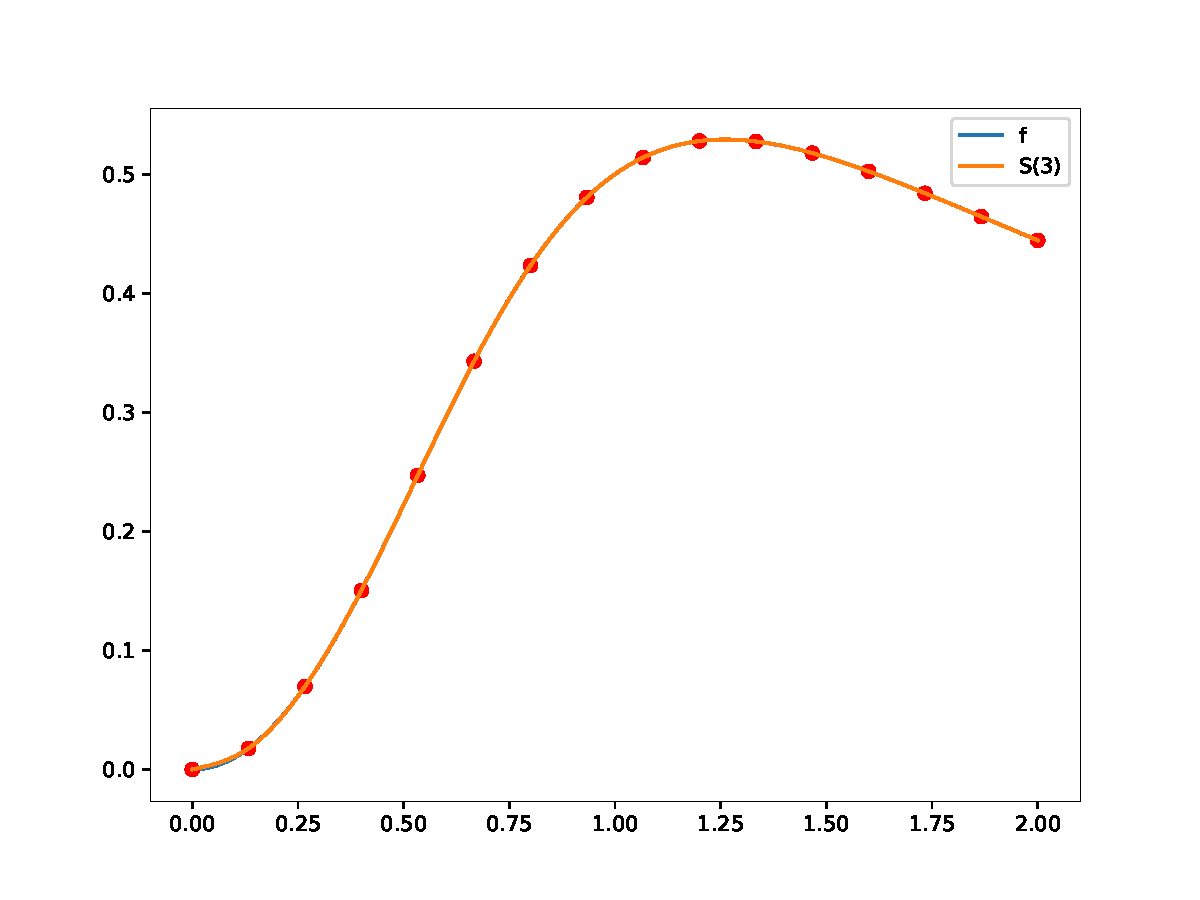
\includegraphics[width=\linewidth]{3.pdf}
	\caption{Третье дополнительное условие}
	\label{fig:case_3}
\end{figure}


\begin{figure}[H]
	\centering
	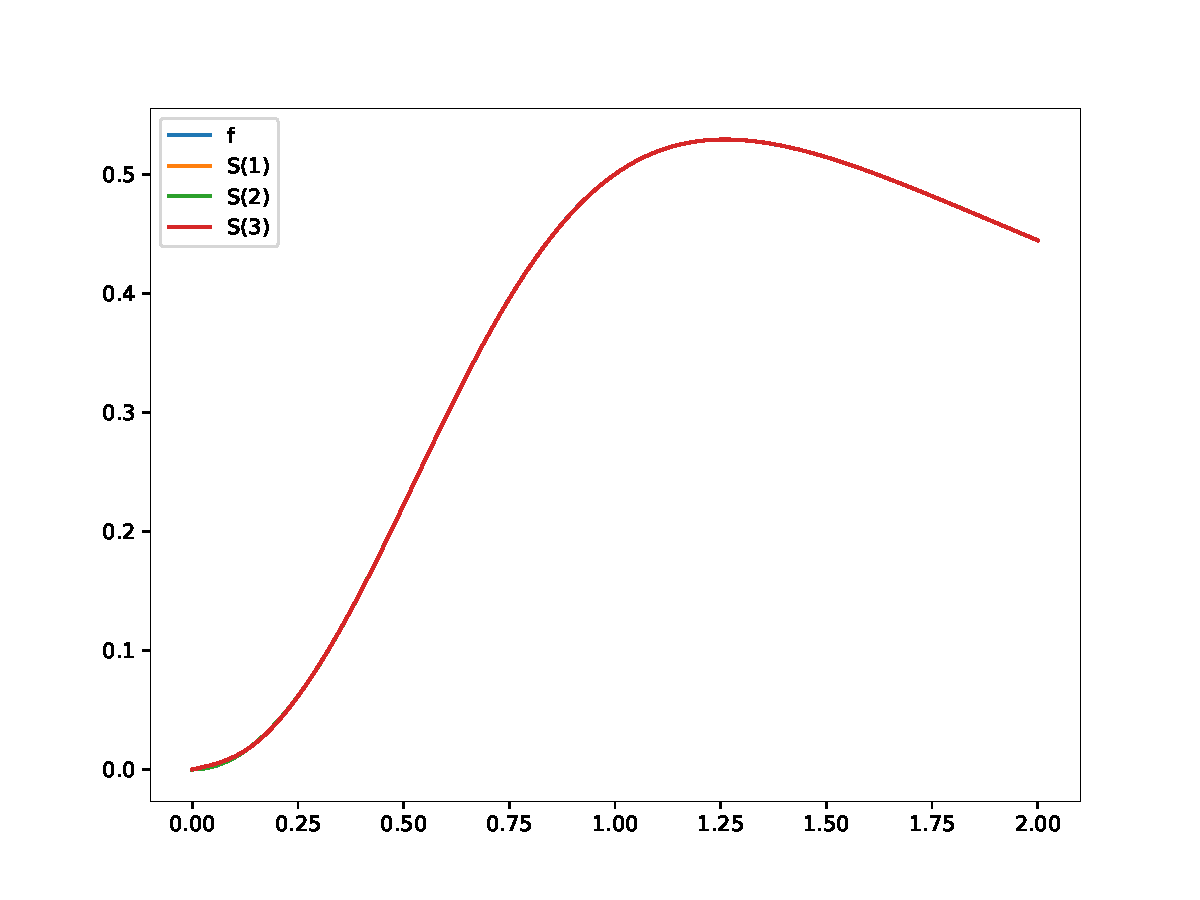
\includegraphics[width=\linewidth]{4.pdf}
	\caption{Все сплайны на одном графике}
	\label{fig:three_cases}
\end{figure}

\begin{table}[H]
	\centering
	\begin{tabular}{|l|l|}
	\hline
		Сплайн	& $\max_{j=0,\ n-1}|f(\overline{x_j}) - S_3(\overline{x_j})|$ \\ \hline
		1   	&     $0.000026258620$	\\ \hline
		2   	&     $0.000026264849$		\\ \hline
		3   	&     $0.001633497939$		\\ \hline
	\end{tabular}
\end{table}


\section{Выводы}

Для задания кубического интерполяционного сплайна необходимо 
определить граничные условия. Из рассмотренных условий, \eqref{eq:condition_3} 
оказалось наиболее простым в реализации, а \eqref{eq:condition_1}, \eqref{eq:condition_2}
обеспечили наименьшую погрешность по критерию \eqref{eq:criteria}.

\end{document}